\subsection{GritBot}
GritBot является коммерческим продуктом компании RuleQuest Research~\cite{GritBotWebPage}. Вместо поиска точек, наиболее сильно отличающихся от остальной выборки, данный метод ищет подмножества, аномальность которых очевидна~\cite{SchwabacherMachLearnAppl}. Метод определяет границы для непрерывных и список возможных значений для дискретных переменных, формируя набор правил классификации. GritBot основан на использовании деревьев решений~\cite{MartinCompUnsupervisedDetectionMethods} и использует алгоритм C4.5~\cite{MLInCyberTrust}, разработанный Джоном Квинланом и описанный им в~\cite{QuinlanC45}.

Для того, чтобы с помощью C4.5 построить дерево решений и применять его, входные данные должны удовлетворять нескольким условиям.

Информация об объектах, которые необходимо классифицировать, должна быть представлена в виде конечного набора признаков (атрибутов), каждый из которых имеет дискретное или непрерывное значение. Такой набор атрибутов называется \textit{примером}. Для всех примеров количество атрибутов и их состав должны быть постоянными.

Множество классов, на которые будут разбиваться примеры, должно иметь конечное число элементов, а каждый пример должен однозначно относиться к конкретному классу. Для случаев с нечёткой логикой, когда примеры принадлежат к классу с некоторой вероятностью, C4.5 неприменим.

В обучающей выборке количество примеров должно быть значительно больше количества классов, к тому же каждый пример должен быть заранее ассоциирован со своим классом. По этой причине C4.5 является вариантом машинного обучения с учителем.

Данный алгоритм рекурсивно разбивает множество объектов на подмножества так, чтобы энтропия полученных подмножеств была минимальна. Лучшее разбиение при этом выбираетя перебором всех возможных вариантов. 

Построение дерева решений в алгоритме C4.5 происходит следующим образом. Пусть имеется $T$ --- обучающая выборка примеров, а $C$ --- множество классов, состоящее из $k$ элементов. Для каждого примера из $T$ известна его принадлежность к какому-либо из классов $C_1\dots C_k$.

На первом шаге имеется корень и ассоциированное с ним множество $T$, которое необходимо разбить на подмножества. Для этого необходимо выбрать один из атрибутов в качестве проверки. Выбранный атрибут $A$ имеет $n$ значений, что даёт разбиение на $n$ подмножеств. Далее создаются $n$ потомков корня, каждому из которых поставлено в соответствие своё подмножество, полученное при разбиении $T$. Процедура выбора атрибута и разбиения по нему рекурсивно применяется ко всем $n$ потомкам и останавливается в двух случаях:
\begin{itemize}
	\item после очередного ветвления в вершине оказываются примеры из одного класса (тогда она становится \textit{листом} дерева, а класс, которому принадлежат её примеры, будет решением листа);
	\item вершина оказалась ассоциированной с пустым множеством (тогда она становится листом, а в качестве решения выбирается наиболее часто встречающийся класс у непосредственного предка этой вершины).
\end{itemize}

Пример дерева решений, построенного алгоритмом C4.5, приведён на рисунке~\ref{fig:spec:DecisionTreeExample}.

\begin{figure}[h]
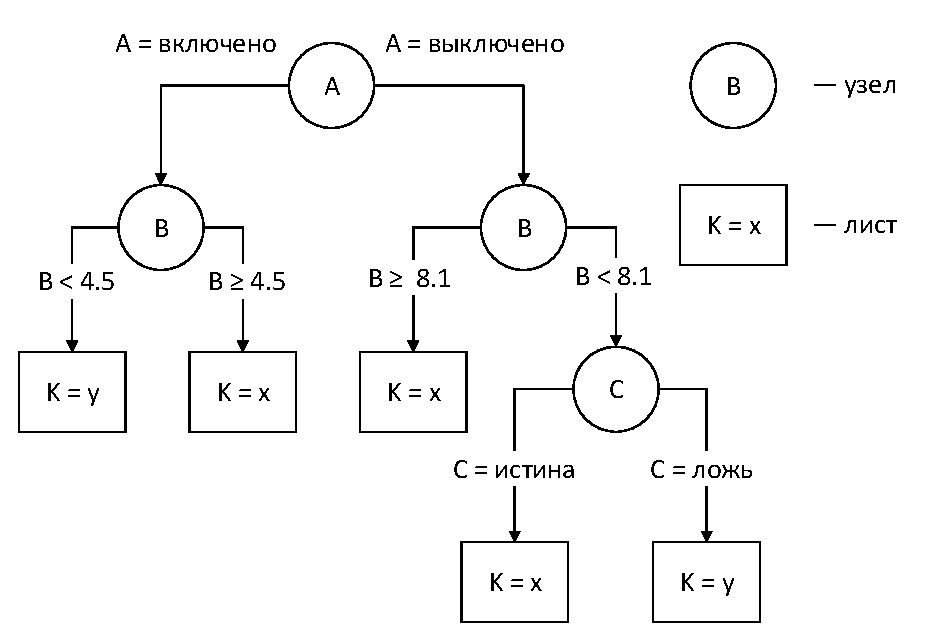
\includegraphics[width=0.7\textwidth, keepaspectratio]{decision_tree}
\caption{Пример дерева решений} \label{fig:spec:DecisionTreeExample}
\end{figure}

Так как алгоритм C4.5 относится к машинному обучению с учителем, GritBot дополняет его механизмом автоматического определения классов на основе вычисления статистических свойств выборки.

В исследовании~\cite{MLInCyberTrust} GritBot показал крайне низкую эффективность, не найдя ни одной добавленной в выборку аномалии. Это связано со статистическим подходим к определению аномальности объекта (метод ищет корреляцию между параметрами объектов в выборке). 

К преимуществам можно отнести лёгкость интерпретации результатов человеком (из-за использования деревьев решений можно получить набор правил, по которым пример был признан аномальным).

Недостатки:
\begin{itemize}
	\item низкая эффективность при наличии в выборке объектов с большим числом аномальных параметров~\cite{MLInCyberTrust};
	\item данный метод загружает весь массив исходных данных в память~\cite{BaySchwabacherOrca}; таким образом, с его помощью невозможно обрабатывать сколь-либо большие выборки;
	\item нет численной оценки степени аномальности примера (метод сортирует аномалии по их статистической значимости)~\cite{MartinCompUnsupervisedDetectionMethods}.
\end{itemize}